\section{Integration: group key agreement protocol with SLP}
There are two main approaches how to integrate a group key agreement protocol into the SLP. It is possible to integrate the group key agreement hardcoded into SLP or as a module adjacent to SLP. Both have benefits and disadvantages. 

\subsection{Hardcoded integration}
With this solution we have to take the SLP specification apart and change many methods to combine a group key agreement protocol with SLP. Such integration means that we need not just some changes but a very new communication workflow with new message formats and timeout behavior. Furthermore the group key agreement protocol couldn't be replaces anymore so all users would be bind to a special group key agreement protocol. That could be a neatly solution but would change the SLP too much and the implementation would be much complicated. Also the SLP wouldn't be compatible to the versions below and that isn't our goal. This approach would deliver a new protocol which probably would scale better as the modular integration solution.

\subsection{Modular integration}
With this solution we don't make many changes in the SLP specification. We use a group key agreement protocol as a module which we combine with SLP without fully integrates it into the SLP specification. In this way the module can easily be replaced anytime. So we are not bound to a special group key agreement protocol. Also it is possible to use many several group agreement protocols at the same time if needed. Our goal was to upgrade the SLP with minimum changes but to solve the requested requirements like discussed in section \ref{sec:conclusion}, so we decided to take this solution. Furthermore this solution can be applied much easier on current SLP implementation as a hardcoded integration.\\
For this purpose we have minor changes in the source code. Like discussed above we took TGDH as our group agreement protocol. To make SLP work with TGDH we had to change the header of SLP messages and implement additional functions into SLP to communicate with our group agreement protocol. A disadvantage of this method is a bigger communication overhead because SLP and the group key agreement protocol don't work synchronized together.

\subsubsection{Workflow of SLP with a modular integration}
\begin{figure*}[!h]
\centering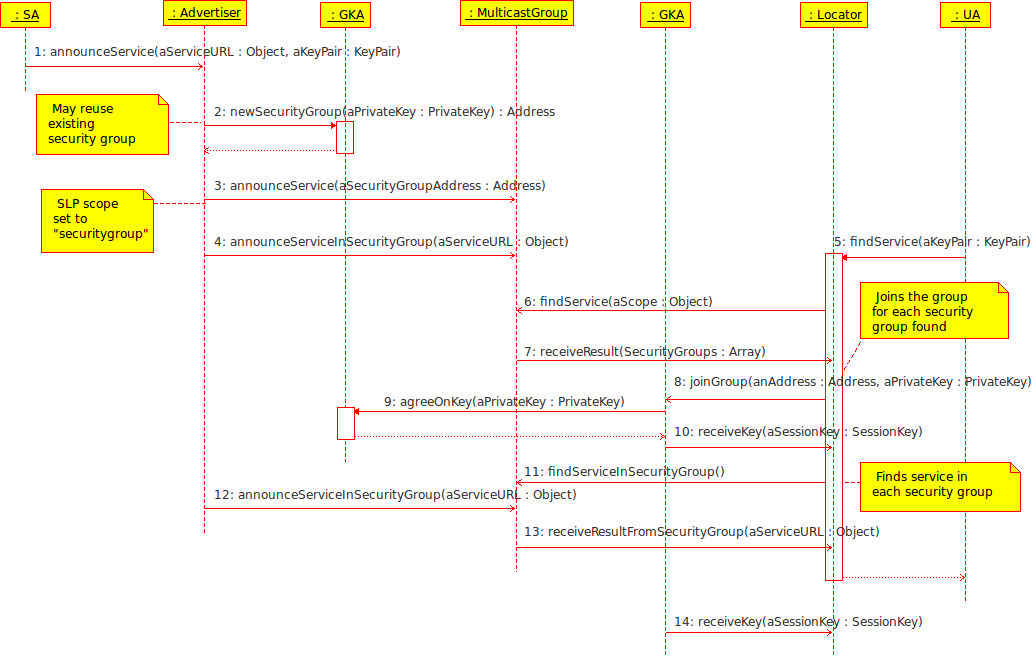
\includegraphics[width=1.0\textwidth]{Images/SequenceDiagramm}
\caption{Sequence diagramm \ldots}
\label{}
\end{figure*}
\textcolor{red}{hier noch ein Bild einf�gen}